%% bare_jrnl.tex
%% V1.4b
%% 2015/08/26
%%
%% Support sites:
%% http://www.michaelshell.org/tex/ieeetran/
%% http://www.ctan.org/pkg/ieeetran
%% and
%% http://www.ieee.org/

%

% *** Authors should verify (and, if needed, correct) their LaTeX system  ***
% *** with the testflow diagnostic prior to trusting their LaTeX platform ***
% *** with production work. The IEEE's font choices and paper sizes can   ***
% *** trigger bugs that do not appear when using other class files.       ***                          ***
% The testflow support page is at:
% http://www.michaelshell.org/tex/testflow/
% git @ /home/srout/Dropbox/educational/Silicon/Journal-preprint/2023-texrxiv-RISCV-Brief-History

%% Feedback from Dr. Chandra Shekhar 04/10/24
% https://www.renesas.com/us/en/products/microcontrollers-microprocessors/risc-v/r9a02g021-ultra-low-power-48mhz-mcu-renesas-risc-v-cpu-core?utm_campaign=s-p-mcu_riscv_gp-epsg-iotbd-ipm1-na&utm_source=google&utm_medium=cpc_txt&utm_content=pp&gad_source=1&gclid=CjwKCAjwoPOwBhAeEiwAJuXRhy32BLt_VCmevFGbn4qpvCAXzaoKXfkDHLAyAejmK6w050wACFcbKRoCqgEQAvD_BwE

\documentclass[journal]{IEEEtran}
%
%
\ifCLASSINFOpdf
  \usepackage[pdftex]{graphicx}
\else
  % DVI stuff 
\fi
%% For citation
\usepackage{cite}
% correct bad hyphenation here
\hyphenation{op-tical net-works semi-conduc-tor}


\begin{document}
%
\title{The Rise and Popularity of RISC-V}
%
\author{Saroj~Rout,~\IEEEmembership{Senior Member,~IEEE}\thanks{Dr. Saroj Rout is with Department of Electronics Engineering, Silicon Institute of Technology, Bhubaneswar, India (https://sroutk.github.io)} and Chandra~Shekhar\thanks{Dr. Chandra Shekhar currently serves as the Professor Emeritus at Birla Institute of Technology \& Science, Pilani, Rajasthan, India} }

% The paper headers
\markboth{Preprints in Technology Research at TechRxiv, January~2024}%
{Rout \MakeLowercase{\textit{et al.}}: The Rise and Popularity of RISC-V}

% make the title area
\maketitle

\begin{abstract}

RISC-V, a Reduced Instruction Set Computer (RISC) architecture has emerged as the architecture of choice for power-conscious devices such as tablets, mobile phones, and IoT embedded systems. This article looks at the evolution of RISC-V to give readers a historical perspective on its enormous success.  

\end{abstract}



% Note that keywords are not normally used for peerreview papers.
\begin{IEEEkeywords}
RISC-V, RISC, Computer Architecture
\end{IEEEkeywords}

%%%%%%%%%%%%%%%%%%%%%%%%%%%%%%%%%%%%%
% INTRODUCTION
%%%%%%%%%%%%%%%%%%%%%%%%%%%%%%%%%%%%%
\section{Introduction}

\IEEEPARstart{S}{ystems-on-a-chip} (SoC) with integrated processors are becoming ubiquitous. One such SoC is a microcontroller. It is hard to find an electronic system without a microcontroller in it, e.g. IoT, appliances, watches, toys, etc. They vary in complexity depending on the target applications. For example, Atmel's ATtiny series of microcontrollers are 8-bit processors starting with just 512-byte Flash and 32-byte SRAM running at 10 MHz clock speed \cite{microchip_attiny85_nodate}. On the other end of the spectrum are the popular STMicroelectronic STM32 series microcontrollers, which are based on Arm's Cortex-M 32-bit processor with up to 128 kB of L2 cache and more than 600 kB of SRAM running at 650 MHz \cite{stmicroelectronics_stm32_nodate}.

%%FIGURE : uC
\begin{figure}[htb]
    \centering
    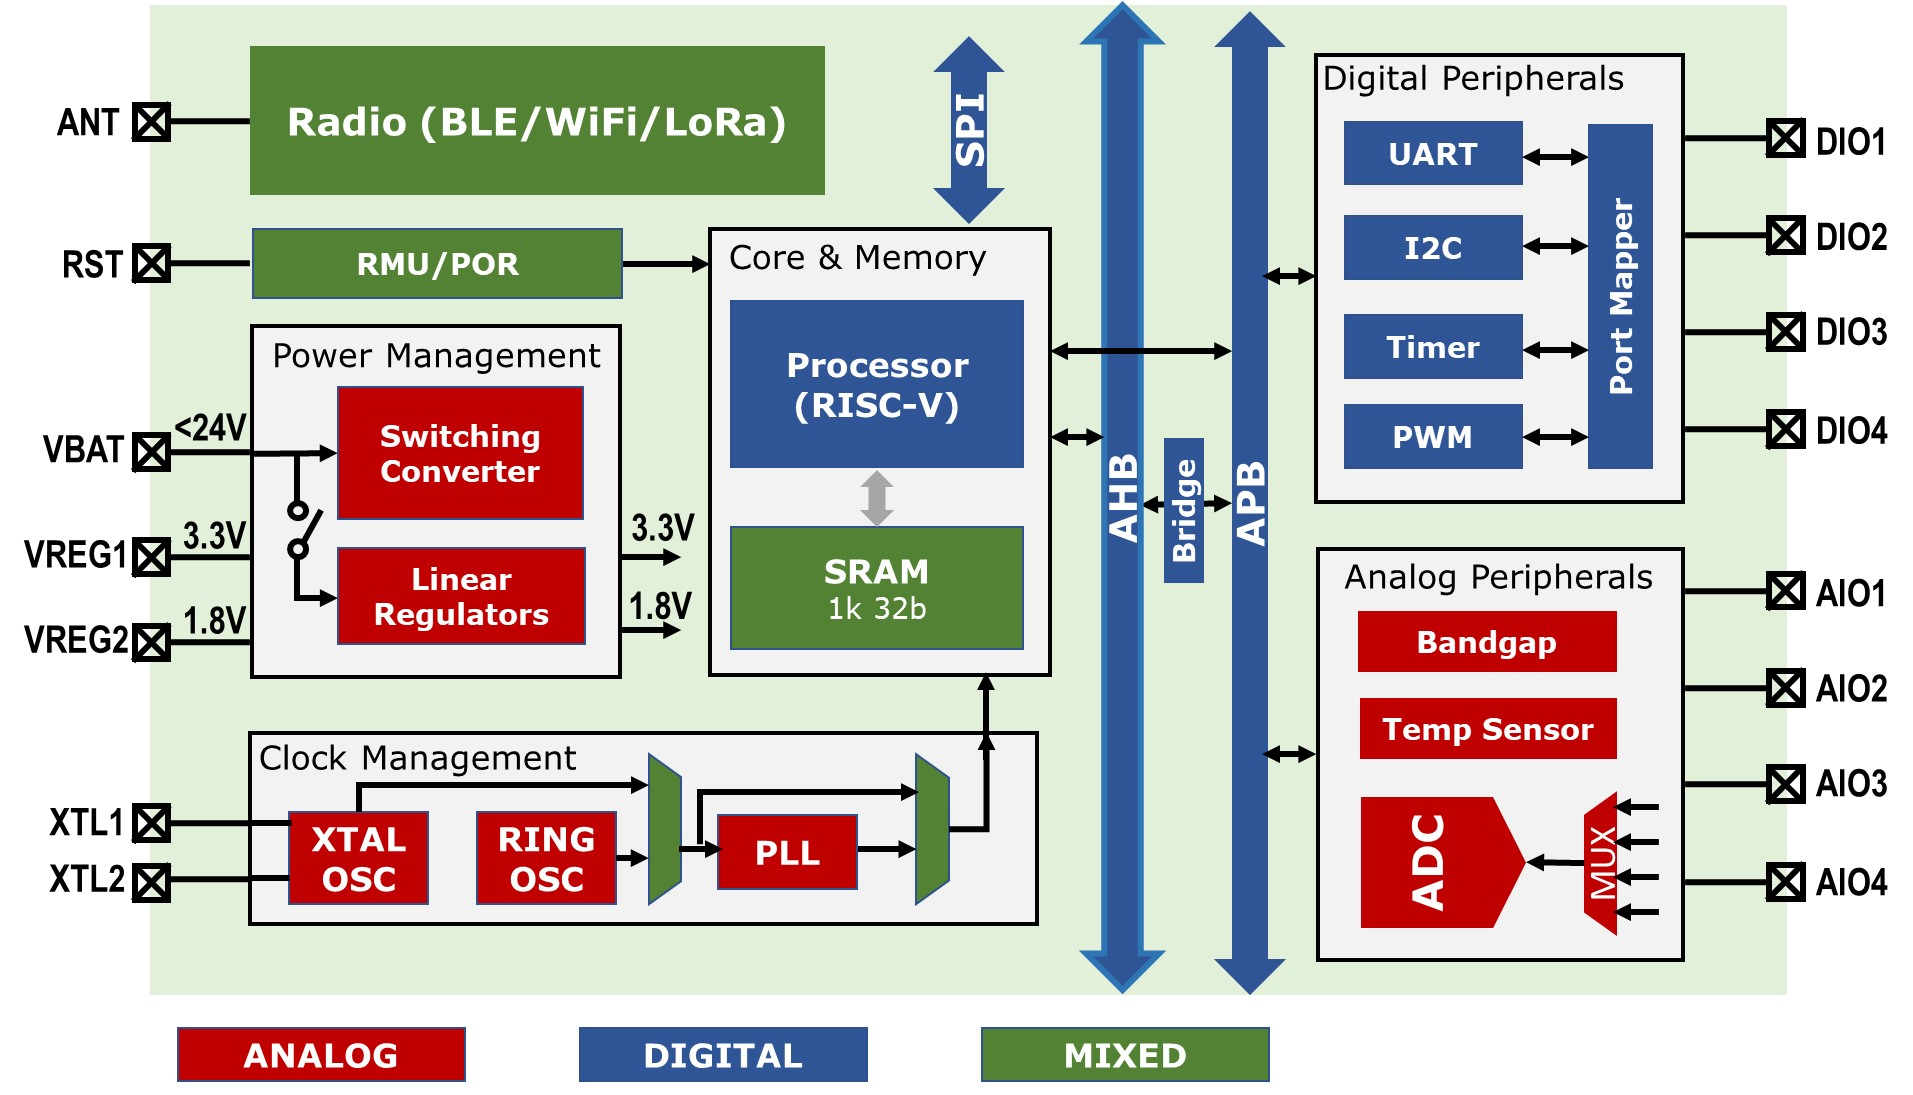
\includegraphics[width=0.95\linewidth]{image-uC.jpg}
    \caption{Architecture of a microcontroller intended for wireless IoT nodes.}
    \label{fig:uC}
\end{figure}

Fig.~\ref{fig:uC} shows an architecture of a microcontroller designed for IoT wireless nodes. It contains a core processor, a cache (SRAM), analog peripherals (bandgap voltage reference, temperature sensor, and analog-to-digital converter(ADC)), digital peripherals (UART, SPI, PWM), power management, clock management (PLL, crystal oscillator) and RF Radio (Bluetooth, WiFi, LoRa \cite{sinha_survey_2017, bor_lora_2016}). Apart from the processor, all other blocks (typically called IPs) can be either designed from scratch by mixed-signal engineers or licensed from a vendor. When it comes to the processor, it becomes a little complicated. You can use a very old instruction set architecture (ISA) and implement it in your target technology. One such popular ISA is Intel's 8051 microcontroller architecture developed in 1980s \cite{noauthor_mcs-51_2023}. It has been around for several decades and has proven to be reliable, efficient, and versatile. Its compact size, low power consumption, and wide range of peripherals make it a popular choice for many embedded system applications. Additionally, there is a large community of developers and engineers who are familiar with the 8051 architecture, making it easier to find support and resources for development.

Companies like Arm, IBM, and Intel have very successful ISAs, but patents on key aspects of their ISAs prevent others from using them without licenses, which imposes a prohibitive cost for most educational, research organization or companies trying to target low-volume markets. 
Note that ISA is not an implementation of the hardware or software (OS, drivers, compilers). It is a standardization of the interface specification, so development tools and design implementations can be reused and shared, provided that they are open and free. And both hardware and software can be implemented in three ways: proprietary, licensed open-source, or free open-source.

There are three free and open-source RISC ISAs currently available for use\cite{asanovic_instruction_2014}:
\begin{enumerate}
    \item \emph{SPARC V8} from Sun Microsystems that was made into a IEEE standard in 1994.
    \item \emph{OpenRISC} is a GNU open-source effort started in 2000, with 64-bit ISA completed in 2011.
    \item \emph{RISC-V} (pronounced "RISC 5") a BSD open-source effort started in 2010 at the University of California at Berkeley by Krste Asanović, David A. Patterson and their graduate students Andrew Waterman and Yunsup Lee partly inspired by ARM's IP restrictions together with the lack of 64-bit addresses and overall baroqueness of ARM v7.
\end{enumerate}

Before we look at the history of RISC-V and why it prospered compared to it's predecessors SPARC V8 and OpenRISC, it is worth taking a quick look at the history of microprocessors and how RISC has emerged as the goto architecture for power-conscious devices such as tablets, mobile phones, and embedded systems.

%%%%%%%%%%%%%%%%%%%%%%%%%%%%%%%%%%%%%
% BRIEF HISTORY OF MICROPROCESSORS
%%%%%%%%%%%%%%%%%%%%%%%%%%%%%%%%%%%%%
\section{Brief History of Microprocessors}

The birth of a microprocessor took place around the end of 1960s when a Japanese calculator maker Business Computer Corporation (Busicom) contracted with Intel, then a small startup, for custom chips for a calculator. That gave birth to Intel 4004 which is widely accepted as the first microprocessor, and that calculator was launched in early 1971 with Intel 4004 in it along with chips for storage and I/O \cite{faggin_history_1996}. In early 1970, Computer Terminal Corporation (CTC), a company based in San Antonio, TX, USA, arranged Intel to build a single MOS chip to replace their discrete-based 8-bit processor for their general-purpose computer, Data Point 2200. Although Intel went ahead and built the chip based on the Data Point 2200 architecture, the project was suspended as CTC contracted Texas Instruments (TI) for the job \footnote{An interesting historical note: Intel was a startup with about 100 employees, and Texas Instruments was a large company with more than 45,000 employees}. TI developed the TMC 1795 processor for CTC which was rejected after testing the chip. Eventually, TI abandoned the project after failing to market it to other companies. In the mean time, Intel 8008 was successfully working at the end of 1971, but CTC had lost interest in that project and gave up its exclusive right to design. Intel then commercialized 8008 in April 1972, and went on to become a successful product. In 1974 the 8008 spawned the Intel 8080, which in turn heavily influenced the Intel 8086 and today's x86 architecture, which went on to dominate the personal computer (PC) and the server market \cite{noauthor_intel_2024}. So the history is certainly very interesting, where it all started with CTC's Data Point 2200 computer, which eventually established Intel as a microprocessor company and its x86 architecture as a leading architecture in the years ahead.

From 1978 until 1988, the complex instruction set computer (CISC) architecture \cite{blem_power_2013} dominated the market, with performance improvement averaging at 15\% per year. This improvement mainly owed to Moore's law, which ensured the doubling of transistors per unit area every 18 months, and Dennard's scaling theory to ensure that the power consumed in the chip also remained about the same.

From 1988-2003, the focus shifted to improving single-processor performance by exploiting instruction level parallelism (ILP), which led to Reduced Instruction Set Computer (RISC) architecture \cite{patterson_risc_1998} becoming mainstream. Single processor performance improved tremendously with the use of pipelining for single-cylce execution, branch prediction, out-of-order execution, on-chip caches, multilevel on-chip caches, superscalar processors, and VLIW. The continuing benefit of Moore's law and the improvement in Dennard scaling performance was averaged at 40 \% per year.
This performance enhancement was the result of the change in the RISC Instruction Set Architecture (ISA) and microarchitectures based on pipelined execution. RISC offered a simplified ISA that restricted arithmetic and logic operations to register operands as source and destination operands. Memory access was limited to two instructions, load and store, without performing any logic or arithmetic operation on the operands. Memory addressing modes were fewer and simpler compared to CISC. The RISC ISA also allowed for ILP through pipelining of instructions that gives a throughput of one instruction per cycle, in contrast to a CISC architecture taking multiple cycles for an instruction to execute. Additionally, RISC ISA also allowed for Superscalar Processing where more than one instruction can be fed to the pipeline in parallel, albeit some challenges involved in doing so.

 
%%%%%%%%%%%%%%%%%%%%%%%%%%%%%%%%%%%%%
% The Emergence of RISC-V as Free, Open ISA 
%%%%%%%%%%%%%%%%%%%%%%%%%%%%%%%%%%%%%
\section{The Emergence of RISC-V as Free, Open ISA }
For an open-source ISA to have a long and successful lifespan, the founders of RISC-V were wise to look for a proven commercial record. This quickly eliminated some unsuccessful ones or those that have slowly died down, including the \textit{ stack} ISA, \textit{VLIW}, Multiflow, and any new CISC ISAs. While 80x86 had dominated the PC market, \textit{RISC-style} load-store ISAs date back to Seymour Cray's CDC 6600 and RISC had dominated the mobile and tablets of the post-PC Era. Therefore, RISC naturally emerged as a free, open ISA. The founders and the community also felt the need to start with a clean slate with a new RISC ISA to correct some of the mistakes of its predecessors. Some of the learning from the mistakes were: \textit{leaving out essentials} such as the byte load / store or the half word load / store in the initial MIPS I, \textit{making the ISA bulky} by including too much like the register windows in SPARC, or \textit{microarchitectural dependent ISA} like the delayed branch in MIPS. 

Given that the longevity of ISA is in decades, it was essential to look at the future technology landscape to predict some essential features of this new ISA. Three technology platforms seemed to dominate: Internet of Things (IoT), Personal Mobile Devices, and Warehouse-Scale Computers (WSCs). To target these technologies, it will be essential to have four key features from the new ISA:
\begin{itemize}
    \item \textit{Base-plus-extension ISA} with a small core set of instructions for cost-sensitive applications, optional extensions with standard ISA additions to customize SoCs, and space for entirely new set of instructions application-specific SoCs.
    \item \textit{Compact instruction set encoding} for cost-sensitive applications such as IoT that require smaller memory.
    \item \textit{Quadruple-precision (QP) as well as SP and DP} support for wide-ranging data size requirements from WSCs to IoT.
    \item \textit{128-bit addressing} as well as \textit{32-bit and 64-bit}.
\end{itemize}

In order to reduce the code size to about 50 to 60\% of RISC-V instructions in a program, RISC-V now has a 16 bit compressed instruction set \cite{waterman_risc-v_2015}. This extension, named “C”, aims to reduce the static and dynamic code size by adding a short 16-bit instruction encoding for common operations. The C extension can be added to any of the base ISAs (RV32, RV64, RV128), and it is compatible with all other standard instruction extensions.

%%FIGURE : Free ISA score table
\begin{figure}[htb]
    \centering
    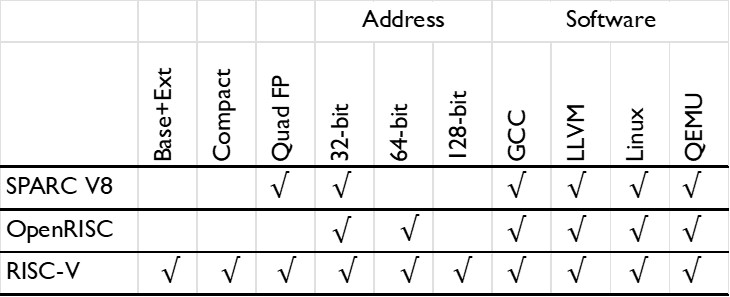
\includegraphics[width=0.95\linewidth]{image-3FreeISA-Table.jpg}
    \caption{Scores for three free open ISAs using four criteria plus listing critical compilers and OS ports.}
    \label{fig:score}
\end{figure}

Fig.\ref{fig:score} tabulates the scores of the three free ISAs based on four criteria plus the list of critical compilers and OS ports. RISC-V meets all the intended requirements while being simple and clean. Because of these advantages, RISC-V gained a lot of momentum among the community and emerged as a clear winner as a choice for a free and open-source ISA. In particular, Chisel \cite{bachrach_chisel_2012} from Berkeley was a highly productive open hardware design system that became part of many silicon successes, making the case for RISC-V even stronger. 
RISC-V continues to evolve, with the 2023 ratification of new specifications including RISC-V Profiles, Volume II Cryptography Extensions, and the IOMMU Architecture Specification \cite{mcmahon_risc-v_nodate}.
%https://riscv.org/announcements/2021/12/risc-v-celebrates-incredible-year-of-growth-and-progress-ratifying-multiple-technical-specifications-launching-new-education-programs-and-accelerating-broad-industry-adoption/

The rise and popularity led to the RISC-V Foundation (www.riscv.org), a nonprofit corporation that was founded in 2015 to build an open and collaborative community of software and hardware innovators based on the RISC-V ISA. In November 2018, the RISC-V Foundation announced a joint collaboration with the Linux Foundation to provide operational, technical, and strategic support.

%%%%%%%%%%%%%%%%%%%%%%%%%%%%%%%%%%%%%
% Latest Advances in RISC-V Technology
%%%%%%%%%%%%%%%%%%%%%%%%%%%%%%%%%%%%%
\section{Latest Advances in RISC-V Technology}
Intel's announcement of a \$1 billion fund to support RISC-V chip development highlights its increasing significance. RISC-V chips are now being used in devices such as earbuds, hard drives, and AI processors, with over 10 billion cores shipped. Companies are also considering RISC-V for data centers and spacecraft \cite{c_chip_nodate}.
%https://www.technologyreview.com/2023/01/09/1064876/riscv-computer-chips-10-breakthough-technologies-2023/
The adoption of RISC-V cores in different industries is predicted to reach 62 billion cores by 2025. A study in 2020 showed almost a quarter of ASIC and FPGA projects incorporating RISC-V cores \cite{redmond_risc-v_2021} and recent trends support this assertion.

Imagination Technologies' RISC-V APXM-6200 CPU, a 64-bit in-order processor with an 11-stage pipeline, is designed for consumer and industrial applications. It offers a high performance density, outperforming the Arm Cortex-A510 in integer performance at similar clock speeds. The inclusion of an SDK with AI libraries, a Visual Studio Code extension, and TEE certification partnerships underscores the increasing adoption of RISC-V in the industry \cite{krewell_imagination_2024}.
%https://www.eetimes.com/imagination-reveals-risc-v-processor-at-embedded-world-2024/

The Titanium Ti375 FPGA by Efinix integrates a quad-core RISC-V, 370,000 logic elements, and features including a Linux-capable MMU, FPU, and custom instructions, making it ideal for AI and edge computing. It also contains a dual transceiver, LPDDR4 DRAM controller, and MIPI D-PHY, all manufactured with 16 nm technology \cite{nordyk_fpga_2024}.
%https://www.edn.com/fpga-integrates-hard-risc-v-cores/

The Roma laptop, the first designed for RISC-V development, features a quad-core 1.5GHz 64-bit CPU, a dual-core GPU, 8GB RAM, 128GB eMMC storage, and a 1TB SSD. It runs on the multilingual openKylin OS, aimed at helping developers create RISC-V software, indicating a significant advancement in the RISC-V ecosystem \cite{ouz_worlds_nodate}.
%http://riscv.org/news/2023/08/worlds-first-risc-v-laptop-roma-officially-delivered-8gb-ram-and-pre-installed-with-domestic-os/

The R9A02G021 MCU, equipped with a 32-bit Renesas RISC-V core, 4 kB of data flash and 16 kB of ECC SRAM, is optimized for energy efficiency and performance. It includes extensive analog features, multiple timers, various serial interfaces, and regulated IOs. Renesas provides a robust ecosystem to support development, highlighting the role of the RISC-V architecture in enhancing design flexibility across industries \cite{noauthor_ultra-low_nodate}.
%https://www.renesas.com/us/en/products/microcontrollers-microprocessors/risc-v/r9a02g021-ultra-low-power-48mhz-mcu-renesas-risc-v-cpu-core

%%Conclusion
\section{Conclusion}
The history thus far has clearly indicated in favor of RISC-V as a free and open ISA. It has created a great opportunity by removing barriers related to design risk, cost of entry, partner limitations, and supply chain. The RISC community took a united approach to learn from previous mistakes of open ISAs and created an ISA for longevity. Given the increasing success of RISC-V, it can be safely envisioned to be the choice of ISA for most power-conscious and those with costs, including IoT, WSC, and mobile devices.  





%%Bibliography
\bibliographystyle{IEEEtran}
\bibliography{2024-RISC-V-techXriv}

% Can use something like this to put references on a page
% by themselves when using endfloat and the captionsoff option.
%\ifCLASSOPTIONcaptionsoff
%  \newpage
%\fi


%\begin{thebibliography}{1}

%\bibitem{IEEEhowto:kopka}
%H.~Kopka and P.~W. Daly, \emph{A Guide to \LaTeX}, 3rd~ed.\hskip 1em plus
%  0.5em minus 0.4em\relax Harlow, England: Addison-Wesley, 1999.
%\end{thebibliography}

% that's all folks
\end{document}


%%*************************************************************************
%% Legal Notice:
%% This code is offered as-is without any warranty either expressed or
%% implied; without even the implied warranty of MERCHANTABILITY or
%% FITNESS FOR A PARTICULAR PURPOSE! 
%% User assumes all risk.
%% In no event shall the IEEE or any contributor to this code be liable for
%% any damages or losses, including, but not limited to, incidental,
%% consequential, or any other damages, resulting from the use or misuse
%% of any information contained here.
%%
%% All comments are the opinions of their respective authors and are not
%% necessarily endorsed by the IEEE.
%%
%% This work is distributed under the LaTeX Project Public License (LPPL)
%% ( http://www.latex-project.org/ ) version 1.3, and may be freely used,
%% distributed and modified. A copy of the LPPL, version 1.3, is included
%% in the base LaTeX documentation of all distributions of LaTeX released
%% 2003/12/01 or later.
%% Retain all contribution notices and credits.
%% ** Modified files should be clearly indicated as such, including  **
%% ** renaming them and changing author support contact information. **
%%*************************************************************************
